\newpage
\begin{recipe}[source={Propia},
portion={4-5 porciones},
preparationtime={\unit[45-50]{m}}
]{Reineta Al Horno Con Papas \\ Rústicas}
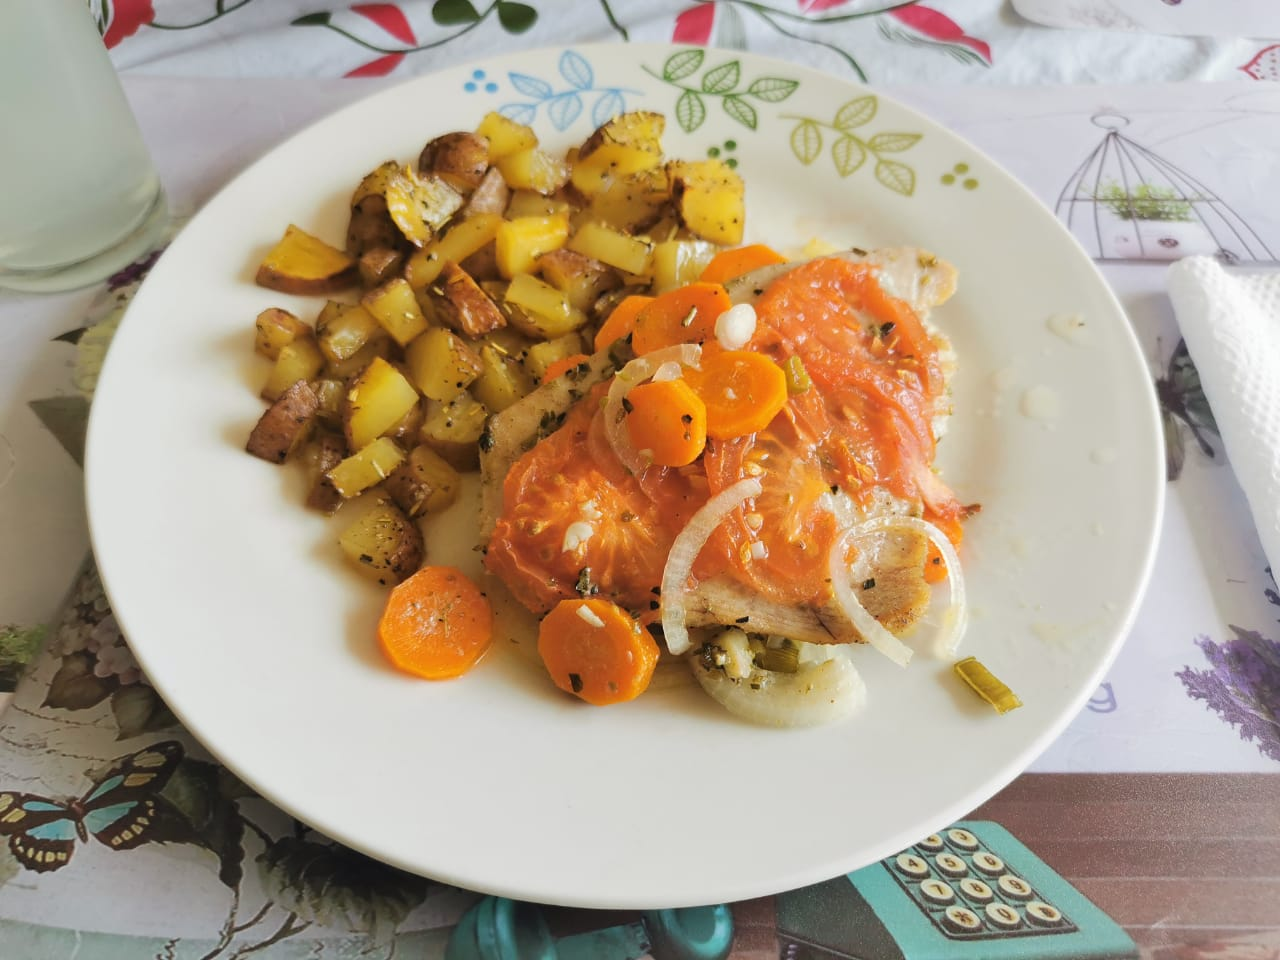
\includegraphics[width=0.25\textwidth]{reineta}
\introduction{
Mi padre solía hacer pescado al jugo en una sartén, en cierta forma me gustaba este plato pero lo adapté al horno para simplificar las cosas, y le agregué algunas cosas de mi cosecha.
}
\ingredients{
    1 & Cebolla cortada en pluma \\
    1 & Cebollín \\
    3 & Dientes de ajo picados finamente \\
    1 & Zanahoria cortada en rodajas \\
    1 & Tomate en rodajas (opcional)\\
    3 & Filetes de reineta \\
    & Sal a gusto \\
    & Pimienta molida a gusto \\
    & Orégano a gusto \\
    & Romero a gusto \\
    & Merquén a gusto \\
    & Ají color a gusto \\
    \unit[80]{gr} & De mantequilla \\
    1 & Copa de vino blanco \\
    & Jugo de limón \\
    4 & Papas \\
}
\preparation{
    \begin{enumerate}
    	\item Precalaentar el horno a 180 grados por 5-10 minutos con calor arriba y abajo.
        \item Enmantequillar la fuente.
        \item Poner abajo la cebolla y luego el cebollin, el ajo picado, la zanahoria, un poco de sal, orégano, pimienta y luego poner el pescado encima.
        \item Poner el tomate encima si es que se optó por el tomate, luego más especias.
        \item Agregar el jugo de limón. 
        \item Agregar la mantequilla encima del pescado en láminas.
        \item Agregar la copa de vino blanco.
		\item En otra fuente, embadurnar con aceite y agregar las papas cortadas y picadas en trozos pequeños.
		\item Agregar romero, merquén, ají color, sal y pimienta a gusto a las papas.
		\item Llevar las papas al horno por aproximadamente 35-40 minutos.
		\item A los 15 minutos restantes de las papas, meter al horno la bandeja con la reineta, y esperar 15 minutos.
		\item Retirar ambas fuentes y servir.
    \end{enumerate}
}
\hint{
	Se puede acompañar con una ensalada a la chilena.
}
\end{recipe}